%\documentclass[dvipdfmx]{beamer}      % platex の場合
\documentclass{beamer}                 % lualatex の場合
\usepackage{mySld}

\begin{document}
\title{基礎コンピュータ工学\\第3章 組み立て\\(パート3)}
\date{}

\begin{frame}
  \titlepage
\end{frame}

%==============================================================================
%\begin{frame}
%  \frametitle
%  \tableofcontents
%\end{frame}

\section{組み立て}
%==============================================================================
\begin{frame}
  \frametitle{LED(ランプ)}
  \vfill
  \centerline{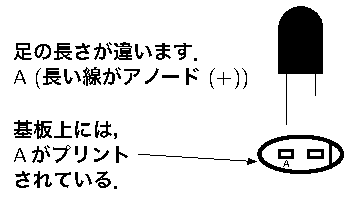
\includegraphics[scale=0.65]{../chap3/leds.pdf}\hspace{2cm}
    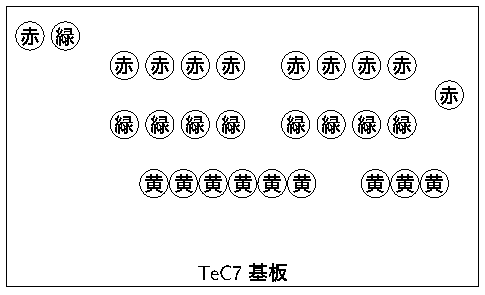
\includegraphics[scale=0.65]{../chap3/leds2.pdf}}
  \vfill
  \begin{enumerate}
    \item[1.] 同じ色を一斉にに,アノード(+)だけハンダ付けする.
    \item[2.] LEDが垂直になっているか確認する.\\
      (垂直になっていない場合は,再度温めて修正する.)
    \item[3.] LEDが奥までささっているか確認する.
    \item[4.] カソードをハンダ付けする.
    \item[5.] リード線を切る.
  \end{enumerate}
  \vfill
\end{frame}

%==============================================================================
\begin{frame}
  \frametitle{スイッチ}
  \vfill
  \centerline{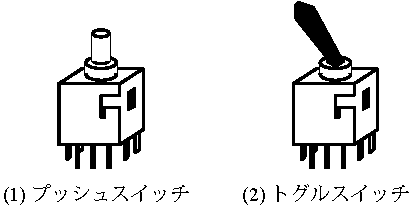
\includegraphics[scale=0.65]{../chap3/sw.pdf}\hspace{1cm}
    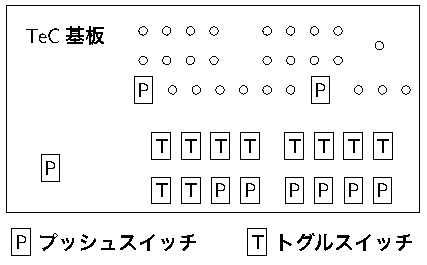
\includegraphics[scale=0.8]{../chap3/sws.pdf}}
  \vfill
  \begin{enumerate}
  \item[1.] 足を穴にしっかり差し込む.
  \item[2.] 足のうち1本をハンダ付けする.
  \item[3.] 一列のスイッチについて1.,2.をする.
  \item[4.] スイッチが傾いていないか確認する.\\
    (傾いていた場合は,温め直して修正する.)
  \item[5.] 他の足をハンダ付けする.
  \end{enumerate}
  \vfill
\end{frame}

%==============================================================================
\begin{frame}
  \frametitle{JTAGコネクタ}
  \centerline{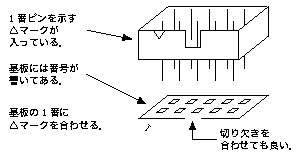
\includegraphics[scale=0.6]{../chap3/cn.pdf}}
  \vfill
  \centerline{\small\begin{tabular}{l|l|l}
      \hline
      \hline
      \multicolumn{1}{c|}{記号} &
      \multicolumn{1}{c|}{型番} &
      \multicolumn{1}{c}{説明} \\
      \hline
      CN4 & なし & 小さい14ピンのコネクタ \\
    \end{tabular}
  }
  \vfill
  \begin{enumerate}
  \item[1.] 向きに注意!!
  \item[2.] 中央付近の一本をハンダ付けする.
  \item[3.] 向き,傾きを再度確認する.
  \item[4.] 残りの足をハンダ付けする.
  \end{enumerate}
  \vfill
\end{frame}

%==============================================================================
\begin{frame}
  \frametitle{入出力ポートコネクタ}
  \centerline{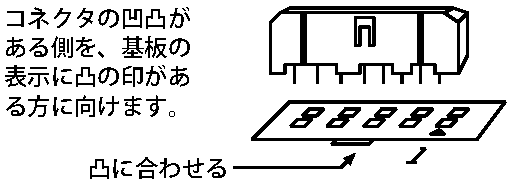
\includegraphics[scale=0.8]{../chap3/cnn.pdf}}
  \vfill
  \centerline{\small\begin{tabular}{l|l|l}
    \hline
    \hline
    \multicolumn{1}{c|}{記号} &
    \multicolumn{1}{c|}{型番} &
    \multicolumn{1}{c}{説明} \\
    \hline
    CN5 & なし & 大きい20ピンのコネクタ \\
  \end{tabular}}
  \vfill
  \begin{enumerate}
  \item[1.] 向きに注意!!
  \item[2.] 中央付近の一本をハンダ付けする.
  \item[3.] 向き,傾きを再度確認する.
  \item[4.] 残りの足をハンダ付けする.
  \end{enumerate}
  \vfill
\end{frame}

%==============================================================================
\begin{frame}
  \frametitle{電源コネクタ}
  \centerline{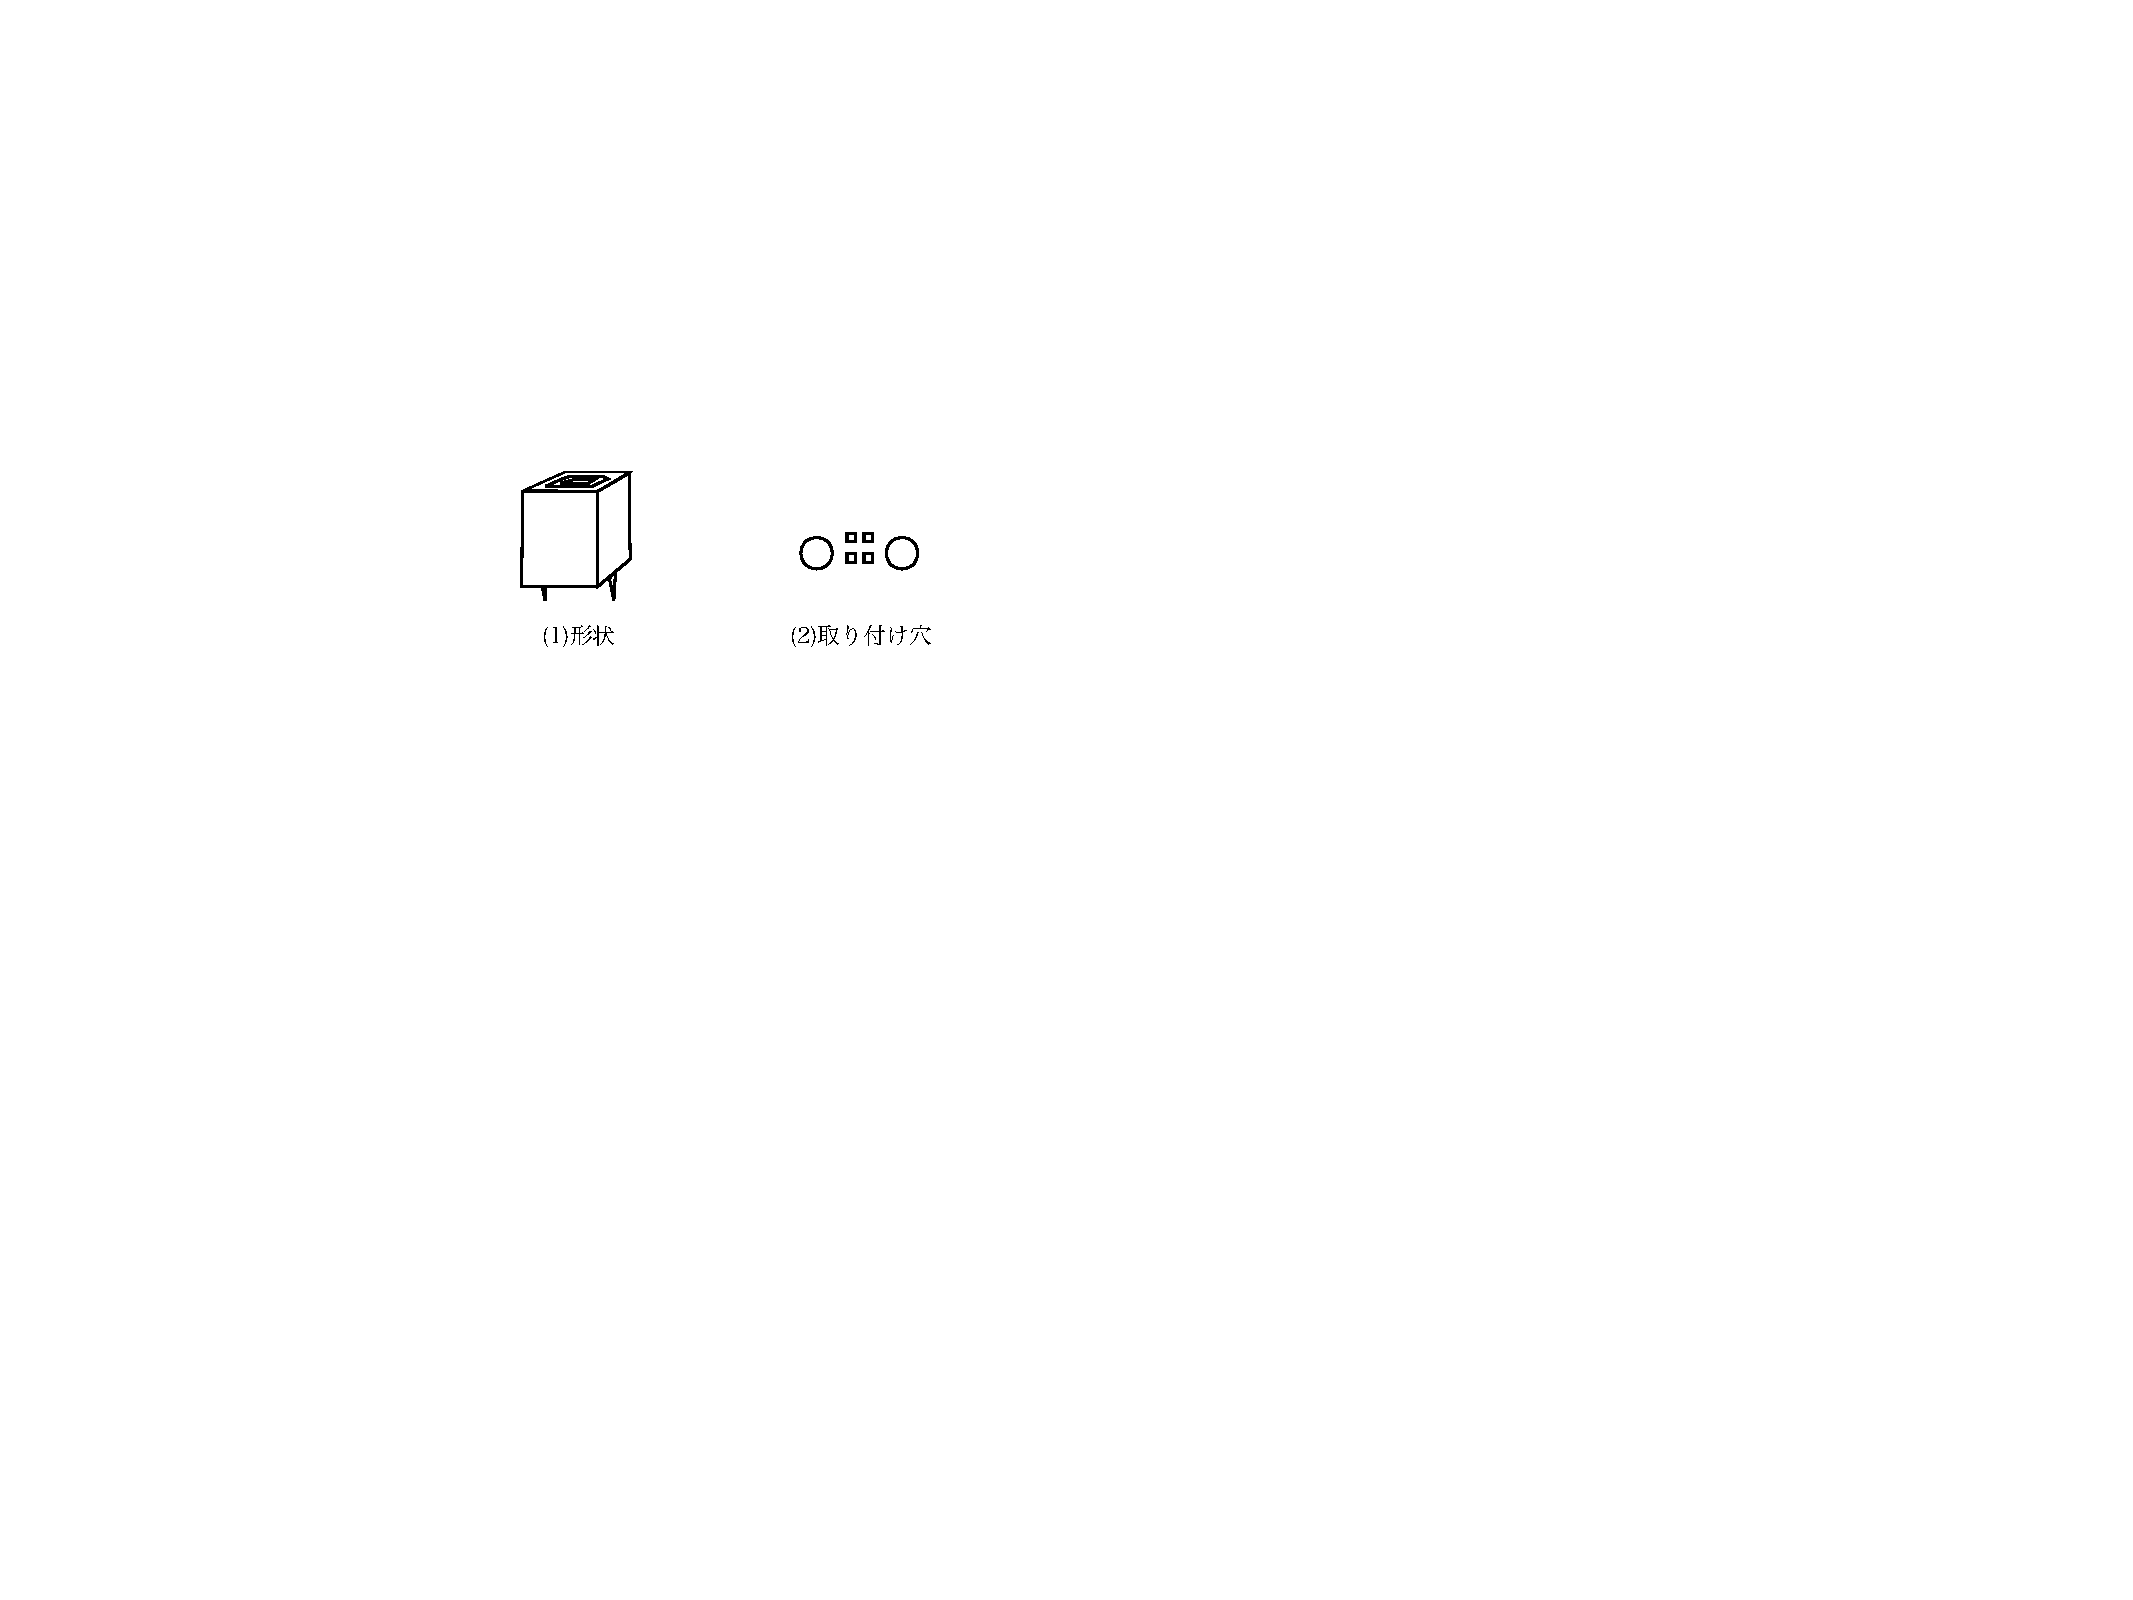
\includegraphics[scale=0.65]{../chap3/cn1.pdf}}
  \vfill
  \centerline{\small\begin{tabular}{l|l|l}
    \hline
    \hline
    \multicolumn{1}{c|}{記号} &
    \multicolumn{1}{c|}{型番} &
    \multicolumn{1}{c}{説明} \\
    \hline
    CN1 & なし & USB-B コネクタ \\
  \end{tabular}}
  \vfill
  \emph{\Large\color{red}やけどに注意!!}
  \begin{enumerate}
  \item[1.] 穴にしっかり差し込む.
  \item[2.] 大きな穴とコネクタの端子を十分熱する.
  \item[3.] 大きな穴が塞がるまで,ハンダをどんどん融かし込む.
  \item[4.] \emph{十分に冷めるのを待つ.}
  \item[5.] 部品が傾いていないか確認する.
  \item[6.] 小さな穴に部品の足をハンダ付けする.
  \end{enumerate}
  \vfill
\end{frame}

%==============================================================================
%\begin{frame}
%  \frametitle{}
%\end{frame}

\end{document}
